\chapter{Introduction}


% \section{Tobacco Addiction and the Challenges of Conventional Talk Therapy}
Tobacco use remains the leading cause of preventable disease and death in Canada. More than 70\% of the lung cancer cases in the country are estimated to be attributable to smoking. Smoking is responsible for the deaths of approximately 45,000 Canadians annually \citep{poirier2019estimates}. Despite public health campaigns and cessation aids, 4.6 million Canadians continue to smoke, with a higher prevalence among Indigenous communities, individuals living in rural areas, and those with low income \cite{cpac2020lung}. These groups also suffer from reduced access to smoking prevention, early diagnosis, and treatment services, which contributes to inequities in health outcomes.

One of the most effective evidence-based interventions for smoking cessation is talk therapy, particularly therapeutic modalities such as cognitive behavioural therapy (CBT) \cite{beck2011cognitive}, acceptance and commitment therapy (ACT) \cite{hayes1999acceptance} and motivational interviewing (MI) \cite{miller2012motivational}. However, access to such interventions is hindered by several systemic challenges. First, traditional talk therapy can be prohibitively expensive for individuals without private insurance or those under financial constraints: although CBT is clinically and economically effective, publicly funded CBT remains scarce in Canada \cite{llewellyn2017economic}. Second, therapy services are limited in availability, especially in rural and remote regions: residents in rural Canada face long distances to providers, transportation difficulties, fewer clinicians, and lower socio-economic resources, all constraining access \cite{crosato2011rural}. Third, there is a significant shortage of culturally safe mental health services tailored to the unique historical and social contexts of Indigenous populations \cite{jones2021mental}. Indigenous communities experience systemic underfunding, long wait times, inadequate provider availability, and cultural mismatches between Indigenous clients and predominantly non-Indigenous therapists \cite{firstnationshealth2023, turner2018poverty}.


One way to address the lack of accessible mental health care is through chatbot-based counselling, which can serve users when no alternatives exist. Chatbots are always available, require no appointments, protect anonymity, and can scale to thousands of users. Once developed, their marginal cost is nearly zero, making them especially suited for underserved populations \cite{torous2017digital,miner2016smartphone}. Compared to traditional therapy, they offer a low-cost, scalable complement.



\section{Motivational Interviewing for Smoking Cessation}

Motivational interviewing (MI) has emerged as particularly effective for smoking cessation. MI is a client-centred counselling method developed in the early 1980s by William R. Miller and later expanded in collaboration with Stephen Rollnick \cite{miller1991motivational,MillerRollnick2013}. It is designed to help individuals 
strengthen their intrinsic motivation to change their health-compromising behaviours, including smoking. MI has been widely applied in addiction treatment settings and has shown consistent effectiveness in encouraging smoking cessation, particularly among individuals not yet ready to quit \cite{bischof2021evidence,hettema2005meta}.

The hallmark of MI is its collaborative, non-confrontational style, which relies on empathy, active listening, and evocation. Rather than telling clients what to do, MI counsellors aim to guide them in articulating their own reasons for change. The core principles of MI are: (1) expressing empathy through reflective listening, (2) developing discrepancy between current behaviour and personal goals, (3) rolling with resistance rather than confronting it, and (4) supporting self-efficacy. \cite{rollnick2008motivational}. These principles are operationalized using skills such as open-ended questions, affirmations, reflections, and summaries---commonly referred to as the OARS model \cite{Miller_2023}.


A critical insight from MI is that \emph{ambivalence} --- a state in which individuals simultaneously hold conflicting feelings about change --- is often the first psychological barrier to change. Smokers may simultaneously recognize the harms of smoking and yet be unwilling to change due to perceived benefits or entrenched habits \cite{brown2023mi}. Resolving this ambivalence is a necessary precursor to behaviour change. Numerous studies have demonstrated that MI increases the number of quit attempts and enhances confidence to quit among ambivalent smokers \cite{Abar2013, Gwaltney2009-wj}. MI promotes a shift from ``sustain talk'' (statements that favour the status quo) to ``change talk'' (statements that favour behavioural change), and the frequency and strength of change talk during a session have been shown to predict actual behavioural outcomes \cite{apodaca2009mechanisms}.

\section{Large Language Models and the Automation of Talk Therapy}
The automation of talk therapy, once constrained to rule-based systems and predefined scripts, has been profoundly transformed by the advent of LLMs. The development of transformer-based architectures \cite{vaswani2017attention}, particularly autoregressive generative models like GPT-3 and GPT-4, has enabled machines to produce responses that are coherent, contextually appropriate, and human-like in natural dialogue \cite{openai2023gpt4}. These capabilities have made fully-generative counselling by LLMs not only possible but increasingly effective for therapeutic applications \cite{miner2020artificial, torous2023generative}.

Several key technical innovations have facilitated the adaptation of LLMs to therapeutic contexts. The self-attention mechanism within transformer models supports long-range dependency modelling and nuanced context tracking across multi-turn dialogues \cite{vaswani2017attention}. Fine-tuning an LLM on domain-specific corpora (e.g., MI transcripts) could make the model outputs clinically grounded \cite{valentino2024evaluating}, while reinforcement learning with human feedback (RLHF) has been shown to improve the relevance, tone, and empathetic quality of generated responses \cite{10.5555/3600270.3602281, gilson2023empathy}. Together, these capabilities enable LLMs to generate novel therapeutic reflections, adhere to evidence-based counselling principles, and adaptively modulate tone.



\begin{figure}[ht]
    \centering
    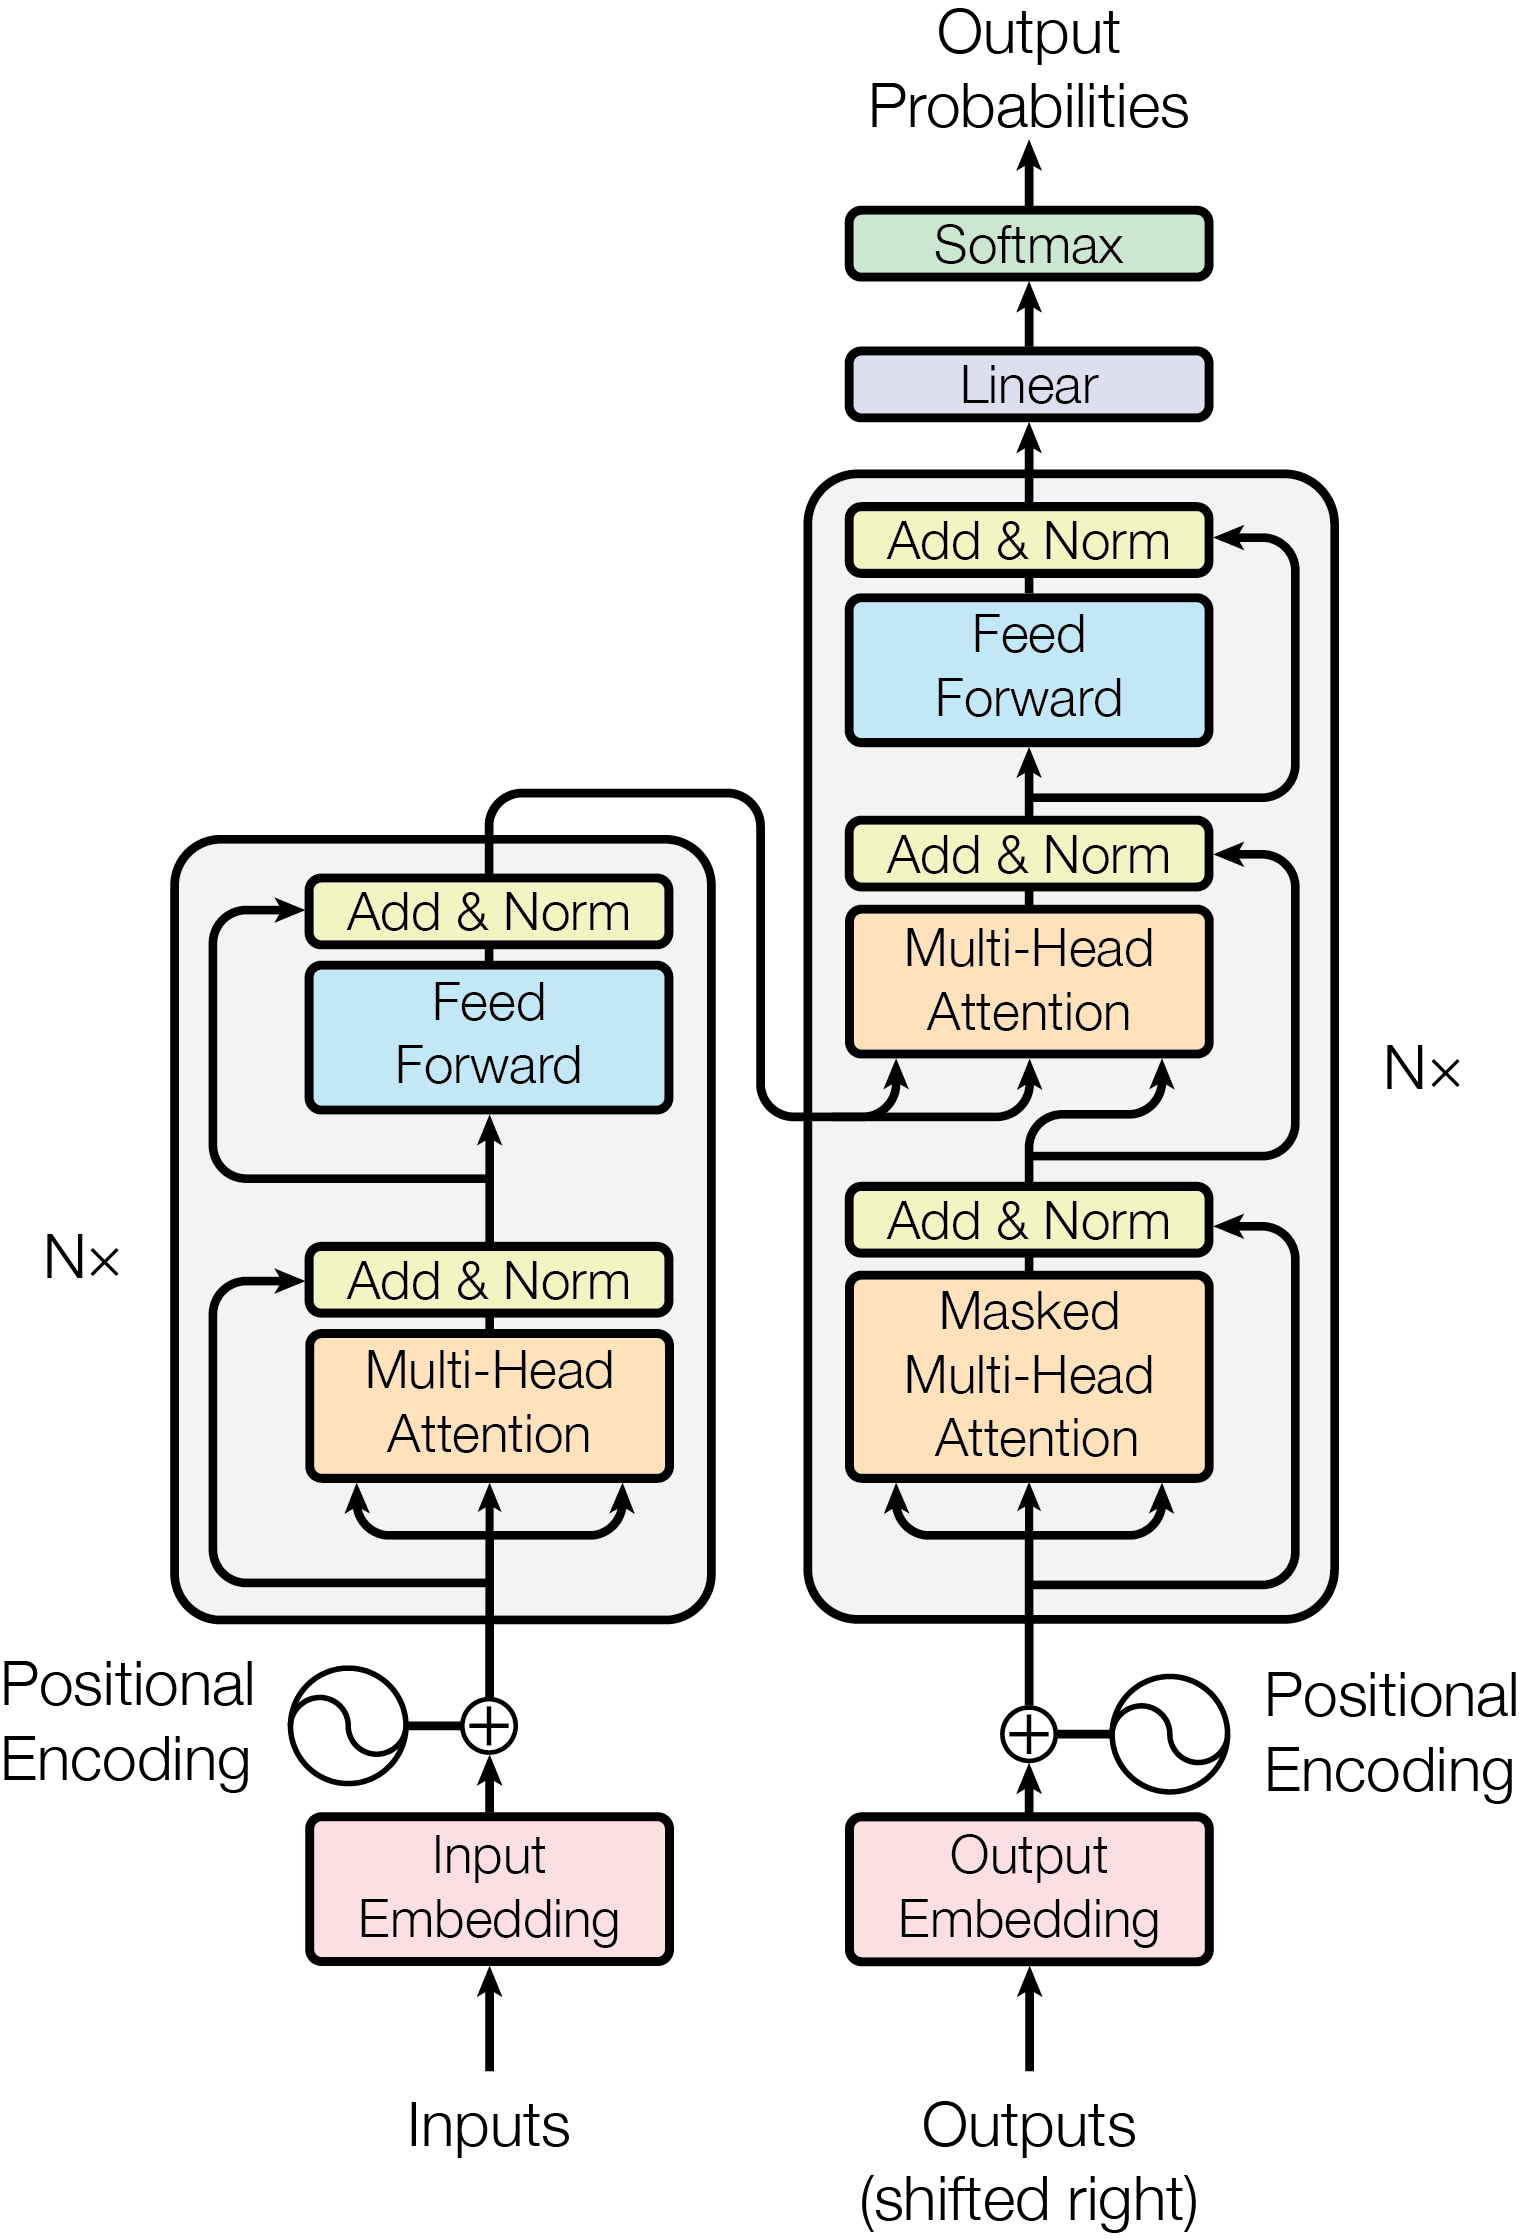
\includegraphics[width=0.6\textwidth]{fig/transformer_architecture.png}
    \caption{Illustration of the Transformer architecture adapted from \citet{vaswani2017attention}.}
    \label{fig:transformer}
\end{figure}


\section{Focus and Goals}
The overarching goal of this project is to develop and evaluate a fully generative chatbot capable of providing MI counselling to help smokers move toward the decision to quit. This involves designing and implementing an MI counsellor that adheres to the core principles of MI, evaluating its effectiveness with real human smokers using both human assessments and automated metrics, and creating \emph{synthetic smokers} --- LLM-based personas that mimic human smokers and consistently display realistic behavioural traits during MI conversations. Furthermore, the realism of these synthetic smokers is validated by comparing their conversational characteristics and behaviours with those observed in actual human smokers. Collectively, these efforts contribute to the broader vision of advancing AI-assisted mental health support through technologies that are safe, accessible, and grounded in evidence-based practices.

\section{Contribution}

This work makes the following contributions to the development and validation of a generative MI-based chatbot for smoking cessation:

\begin{enumerate}
    \item Design and iterative refinement of a single-prompted, fully generative chatbot capable of conducting motivational interviews with human smokers.
    
    \item Execution of an empirical study in which compensated human participants interacted with the chatbot, providing qualitative feedback and pre- and post-interaction self-reports on their readiness to quit smoking. 
    
    \item Development of a methodology to construct \emph{synthetic smokers}—LLM-driven agents embedded with the demographic and behavioural characteristics of human smokers.
    
    \item Creation of evaluation techniques to assess the extent to which these synthetic agents approximate human smokers in controlled behavioural experiments.
    
    \item Validation of synthetic smokers by quantifying their similarity to human smokers using the aforementioned evaluation techniques. 
    
\end{enumerate}

\section{Organization}

This dissertation is structured as follows: Chapter~\ref{ch:background} reviews relevant background on the Motivational Interviewing approach, foundational language models, chatbots for talk therapy, persona construction using LLMs, and prior work on the development and validation of LLM-based synthetic subjects in behavioural experiments. Chapter~\ref{ch:mibot} presents the design of the fully generative MI counselling chatbot, along with details of its deployment and evaluation methodology. Chapter~\ref{ch:mibot-eval} reports the results of a study in which recruited smokers interacted with the chatbot. Chapter 5 describes a method for constructing synthetic smokers using large language models, prompted to exhibit demographic and behavioural traits derived from real smokers. Chapter 6 introduces a framework for evaluating synthetic smokers in their ability to substitute for human participants in controlled behavioural studies, and presents the corresponding evaluation results. Chapter 7 concludes the work by discussing its limitations and outlining directions for future research.
